\subsection{Efficienza locale}
\label{localis}
Utilizzando gli stessi dati della \autoref{attenu}, abbiamo studiato le variazioni di efficienza in vari punti del PM1. In \autoref{capolavoro} è presente un grafico 3D che mostra i conteggi ottenuti in ogni casella in cui è stato posizionato il miniscint. Si può apprezzare una diminuzione dei conteggi tra le varie colonne per i motivi discussi in \autoref{attenu} ma è anche evidente come all'interno di una stessa colonna ci siano delle variazioni significative tra una riga e l'altra.

Per meglio comprendere la situazione, dividiamo tutti i conteggi per quello più alto,
in modo da vedere le variazioni percentuali tra una casella e l'altra del PM1.
La \autoref{auto} riporta i valori dei singoli punti con il loro errore.

\begin{figure}[h]
	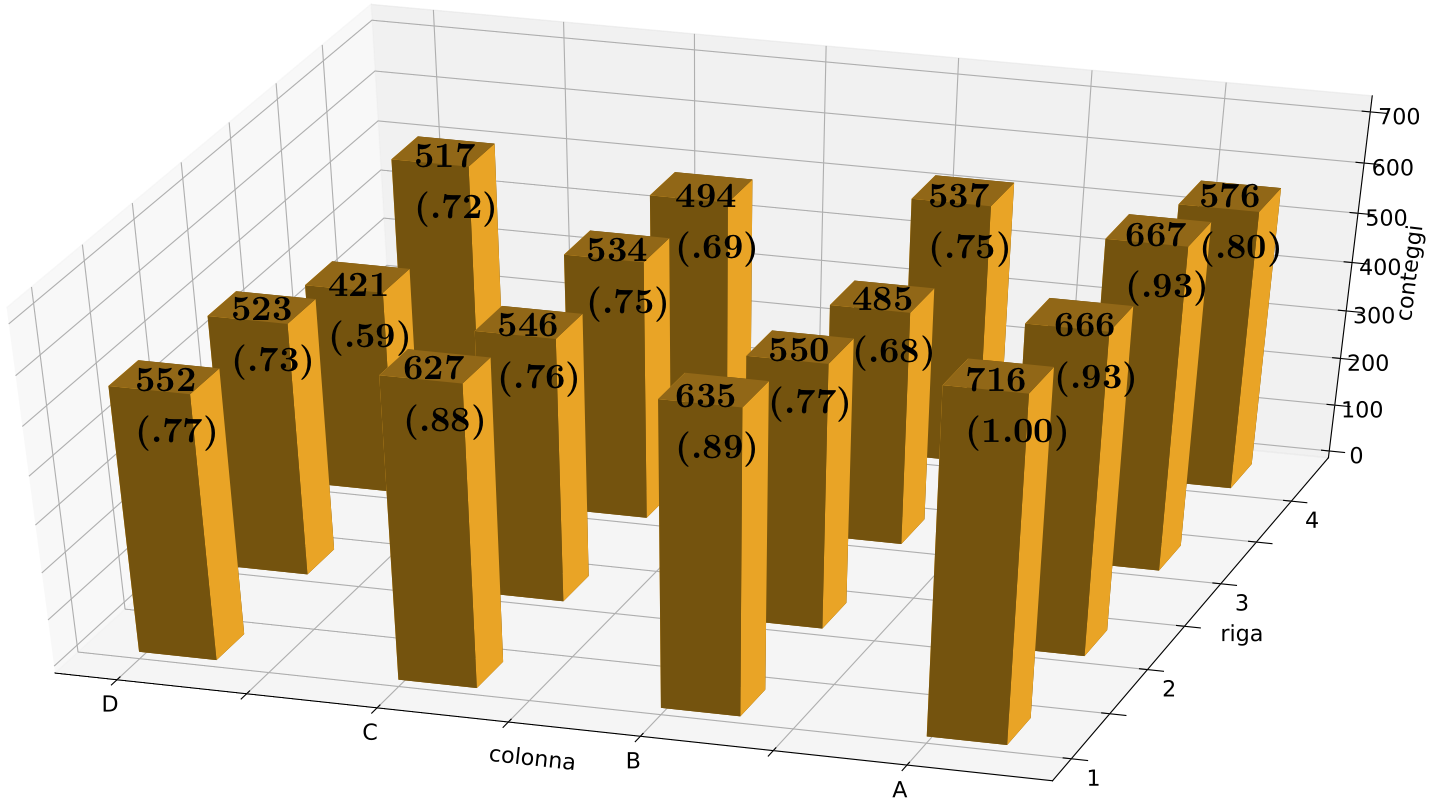
\includegraphics[width=\textwidth]{3d_grande}
	\caption{Conteggi in coincidenza PM1 \& miniscint nelle rispettive caselle.
	Tra parentesi è riportato il valore normalizzato in modo il conteggio più alto valga~1.}
	\label{capolavoro}
\end{figure}

\begin{table}[h]
\centering
\begin{tabular}{|c|c|c|c|c|}
\hline
colonna & D & C & B & A \\
 \hline
riga  & & & &  \\
1 &  $ 0.77 \pm 0.04 $ & $ 0.88 \pm 0.05 $ & $ 0.89 \pm 0.05 $ & $ 1 \pm 0 $ \\ 
2 &  $ 0.73 \pm 0.04 $ & $ 0.76 \pm 0.04 $ & $ 0.77 \pm 0.04 $ & $ 0.93 \pm 0.05 $ \\ 
3 &  $ 0.59 \pm 0.04 $ & $ 0.75 \pm 0.04 $ & $ 0.68 \pm 0.04 $ & $ 0.93 \pm 0.05 $ \\ 
4 &  $ 0.72 \pm 0.04 $ & $ 0.69 \pm 0.04 $ & $ 0.75 \pm 0.04 $ & $ 0.80 \pm 0.05 $ \\
\hline 
\end{tabular}
\caption{conteggi normalizzati nelle varie caselle del PM1.
MODIFICA: dividere per il valore nominale nominale del conteggio massimo in modo che non ci sia la correlazione negli errori.}
\label{auto}
\end{table}
